\section{Lösungsidee}
\begin{wrapfigure}{r}{0.35\textwidth}
  \centering
  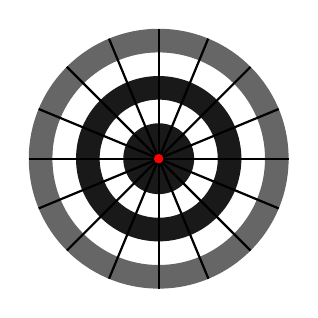
\begin{tikzpicture}[scale=0.3]
	\fill[black!90!white] (0,0) circle [radius=1.5];
	\fill[black!90!white, even odd rule] (0,0) circle[radius=2.5] circle[radius=3.5];
	\fill[black!60!white, even odd rule] (0,0) circle[radius=4.5] circle[radius=5.5];

	\foreach \angle in {0, 22.5, 45, 67.590, 90, 112.5, 135, 157.5, 180, 202.5, 225, 247.5, 270, 292.5, 315, 337.5} 
    	\draw[thick] (0,0) -- (\angle:5.5);

	\fill[red] (0,0) circle[radius=0.2];
\end{tikzpicture}

  \caption{Geraden der Kreisringsegmente}
  \label{abb:spidergrafik}
\end{wrapfigure}
Zunächst habe ich den \task{} mit TikZ nachgezeichnet, um den genauen Aufbau durch Nachbau zu verstehen. Die 16 gleichgroßen Kreissegmente sind durch Geraden getrennt, die im Abstand von \(22,5^{\circ}\) vom Pol (dem Mittelpunkt) aus gezeichnet werden.

Für die Dekodierung stehen mir aus dem Kreismittelpunkterkennungsprozess noch folgende Informationen zur Verfügung: Ein Liste der Kreismittelpunkte und der Kreisdurchmesser. Die Kreisdurchmesser entsprechen der Länge der Zusammenhangskomponenten an den Mittelpunktskoordinaten. Aus diesen Informationen kann ich dank bekannter Proportionen eines \task{}s auf die Positionen der Ringe schließen (siehe Abb. \ref{abb:dims}). Wie in der Lösungsidee zur Kreismittelpunkterkennung festgestellt, beträgt gilt \(u=\frac{1}{3}d\).

\begin{figure}[!ht]
	\centering	
	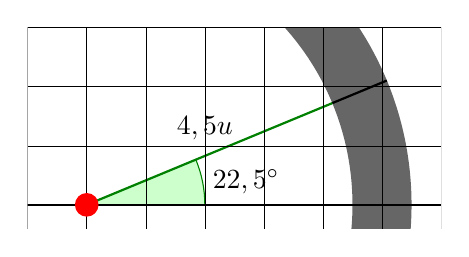
\begin{tikzpicture}[scale=0.75]
	\clip (-1,-0.4) rectangle (6, 3);
	\fill[black!60!white, even odd rule] (0,0) circle[radius=4.5] circle[radius=5.5];

	\foreach \angle in {0, 22.5, 45, 67.590, 90, 112.5, 135, 157.5, 180, 202.5, 225, 247.5, 270, 292.5, 315, 337.5} 
    	\draw[thick] (\angle:4.5) -- (\angle:5.5);

	\filldraw[fill=green!20,draw=green!50!black] (0,0) -- (2,0) arc[start angle=0, end angle=22.5, radius=2];
	\draw[green!50!black, thick] (0,0) -- (22.5:4.5);

	\draw (2, 1.3) node {\(4,5u\)};
	\draw (2.7, 0.4) node {\(22,5^{\circ}\)};

	\draw[very thin] (-6, -6) grid (6, 6);
	\draw[thick] (-6, 0) -- (6, 0);
	\fill[red] (0,0) circle[radius=0.2];
\end{tikzpicture}
	\caption{Punkt einer Gerade, eine Kästchenseite entpricht einem \(u\)}
	\label{abb:trigon}
\end{figure}

Insbesondere kann ich mithilfe von polaren Koordinaten\footnote{\url{https://www.lernhelfer.de/schuelerlexikon/mathematik-abitur/artikel/polarkoordinatensystem}} die Strecken, die die Kreisringe in Segmente einteilen, bestimmen. Jede der Strecken ist ein Teile einer Geraden, die vom Mittelpunkt ausgehend in einem Vielfachen von \(22,5^{\circ}\) durch den Kreis läuft. Die eigentlichen Strecken, die auf dem Kreisring liegen, beginnen nach einem Abstand von \(4,5u\) und enden bei \(5,5u\). Die Punkte aller Strecken lauten also:

\begin{displaymath}
A(k:4,5u) \hspace{2em} B(k:5,5u) \hspace{2em} k := \{22,5 \cdot x \in \mathbb{N}_0 \cup 0 \le x \le 359\}
\end{displaymath}

Nun können wir diese Koordinatenmenge unter Ausnutzung der Regeln im rechtwinkligen Dreieck (s. Abb \ref{abb:trigon}) die kartesischen Koordinaten bestimmen. Das Koordinatensystem ist in der bereits definierten Einheit \(u\).

\begin{gather}
k := \{22,5 \cdot x \in \mathbb{N}_0 \cup 0 \le x \le 359\} \\
\begin{split}
x &= cos(k) \cdot 4,5 \\
y &= sin(k) \cdot 4,5
\end{split}
\hspace{5em}
\begin{split}
x &= cos(k) \cdot 5,5 \\
y &= sin(k) \cdot 5,5
\end{split}
\end{gather}

Da es sehr schwer ist, mit Kreisringsegmenten zu rechnen, nehme ich auch hier eine Vereinfachung vor: Mit den Punkten der segmentbegrenzenden Strecken mit den äußeren Umrandungen des Kreisringes lässt sich 16 Trapeze aufspannen, die den Großteil der Kreissegmente abdecken.:
\begin{figure}[!ht]
	\centering	
	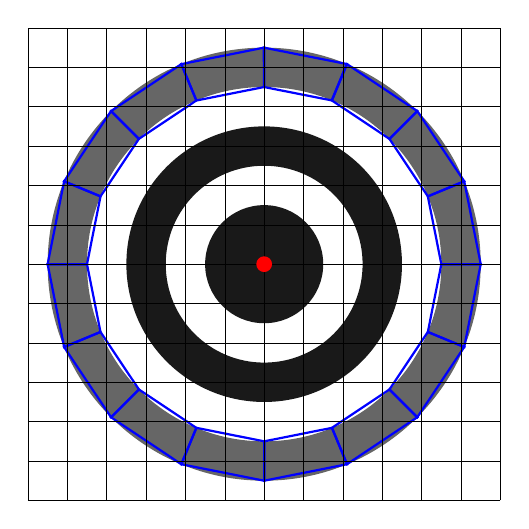
\begin{tikzpicture}[scale=0.5]
	\fill[black!90!white] (0,0) circle [radius=1.5];
	\fill[black!90!white, even odd rule] (0,0) circle[radius=2.5] circle[radius=3.5];
	\fill[black!60!white, even odd rule] (0,0) circle[radius=4.5] circle[radius=5.5];

	\foreach \angle in {0, 22.5, 45, 67.590, 90, 112.5, 135, 157.5, 180, 202.5, 225, 247.5, 270, 292.5, 315, 337.5} 
    	\draw[blue, thick] (\angle:4.5) -- (\angle:5.5) -- (\angle+22.5:5.5) -- (\angle+22.5:4.5) -- cycle;

    	
	\draw[very thin] (-6, -6) grid (6, 6);
	\fill[red] (0,0) circle[radius=0.2];
\end{tikzpicture}
	\caption{Einteilung der 16 Kreisringsegmente in 16 Trapeze}
\end{figure}
\section{Umsetzung}
\section{Beispiele}